The protocol's implementation was done in Java 1.8 and by using the Peersim framework such to be able to perform test on large scale networks. Peersim was chosen among other possible solutions (like AKKA \cite{thurau2012akka}) because of its simplicity and scalability. As a matter of fact, we were unable to replicate such large system with other frameworks because they caused too much overhead.
The source code used is available on Github (\href{https://github.com/geektoni/whanau-sybil-proof-DHT}{https://github.com/geektoni/whanau-sybil-proof-DHT}) such to encourage peer-review and replicability of our results from other researchers.

\subsection{Configuration Parameters}

In order to replicate exactly the experiment done in the original paper, we adopted the same configuration parameters. Table \ref{table:social_network} shows the social network configurations.
Moreover, since we wanted to provide an highly customizable architecture, such to be able to test several possible scenarios, we also provided some additional parameters:
\begin{itemize}
    \item \textbf{layers}: the total number of layers $l$ used by each node;
    \item \textbf{database\_size}: the number of entries $(key,value)$ stored by each node (the default is 1);
    \item \texbf{degree\_node}: the starting degree of the node used by the synthetic graph generator;
    \item \textbf{target\_node}: the target node we want to find using the \textsc{lookup} procedure;
\end{itemize}

\begin{table}[h]
\centering
\caption{Social Network Parameters}
\label{table:social_network}
\begin{tabular}{|l|l|p{5cm}|}
\hline
           & \textbf{Magnitude} & \textbf{Description}                                         \\ \hline
\textit{n} & $n \geq 1$         & Number of honest nodes                                       \\ \hline
\textit{m} & $O(n)$             & Number of honest edges                                       \\ \hline
\textit{w} & $O(\log(n)$        & Mixing time of the honest region (length of the random walk) \\ \hline
\textit{g} & $O(n/w)$   & Number of attack edges                                       \\ \hline
\end{tabular}
\end{table}

\subsection{Package Structure}
Following the Peersim programming model, we developed several Java classes which are used by the \texttt{peersim.CDSimulator} to run the algorithm (Figure \ref{fig:package_structure} shows the package structure).

\subsubsection{Protocol} The only protocol we implemented was the \texttt{WhanauProtocol}. It contains all the routing tables defined before which are used by Whanau. It also contains several helper methods which are used by the \textsc{setup} and \textsc{setup} procedures.

\subsubsection{Controls} We implemented three controls which are used to build the DHT and then to perform the \textsc{lookup} actions:
\begin{itemize}
    \item \texttt{WhanauSetup}: this control is run only once at the beginning of the simulation and it is used to build the initial structure of Whanau. It basically contains the implementation of the \textsc{setup} method outlined above;
    \item \texttt{WhanauWireNetwork}: this control is used to generate the social network topology. It can easily build a random topology using the \textbf{Barabàsi-Albert method} \cite{barabasi1999emergence} or it can process an existing social graph (e.g. DBLP, Youtube, etc.).
    The link protocol used was the already available \texttt{IdleProtocol}, since we did not need advanced or custom functions;
    \item \texttt{WhanauLookup}: this control implements the \textsc{lookup} procedure of Whanau. It is used to test the performance of the protocol under several conditions of the network.
\end{itemize}

\subsubsection{Observers} Besides using the already available observers provided by Peersim, we implemented two additional classes, \texttt{KeyDistributionObserver} and \texttt{WhanauObserver}. The former is used to display the distribution of the IDs over the several layers (in order to check visually for clustering attacks). The latter is used to simply print informations about a given node (its internal tables content).

\begin{figure}[h]
    \centering
    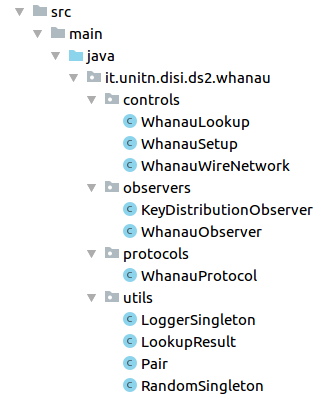
\includegraphics[scale=0.4]{package_structure.png}
    \caption{Java Package Structure of Whanau.}
    \label{fig:package_structure}
\end{figure}